\documentclass[main.tex]{subfiles}
\begin{document}

\chapter{Algoritmes}
\label{cha:algoritmes}

\section{Integreren over twee veranderlijke met een onderling afhankelijk domein}
\subsection*{Abstract}
\subsubsection*{Vraag}
Gegeven een functie $f$ in twee veranderlijken:
\[ f:\ A \subseteq \mathbb{R}^{2} \rightarrow \mathbb{R}:\ (x,y) \mapsto f(x,y) \]
Zij $P$ het predicaat dat bepaalt of een koppel $(x,y)\in\mathbb{R}^{2}$ tot $A$ behoort.
\[ \forall (x,y) \in \mathbb{R}^{2}:\ (x,y)\in A \Leftrightarrow P(x,y) \]
$A$ is dan gedefinieerd als volgt:
\[ A = \{ (x,y) \mid P(x,y) \} \]
Bereken de volgende integraal:
\[ \int_{(x,y)\in A}f(x,y)\ dx dy \]

\subsubsection*{Antwoord}
We zullen proberen de integraal op te splitsen in twee integralen.
We hebben daarvoor een aangepaste versie van het predicaat $P$ nodig, namelijk het predicaat $P_{x}$ of $P_{y}$.
$P_{y}(x)$ is het predicaat dat voor een gegeven $y$ bepaalt of een $x$ tot $A$ behoort:
\[ \forall (x,y) \in \mathbb{R}^{2}:\ (x,y)\in A \Leftrightarrow P_{y}(x) \]
Aan de hand van $P_{y}(x)$ of $P_{x}(y)$ kunnen we respectievelijk $A_{y}$ en $A_{x}$ definieren:
\[ A_{y} = \{ (x,y) \mid P_{y}(x) \} \]
Eveneens defini\"eren we $E_{X}$ en $E_{Y}$ als volgt:
\[ E_{X} = \{ x \in\mathbb{R} \mid \exists y \in \mathbb{R}:\ P_{y}(x) \} \]
We kunnen nu de integraal splitsen:
\[ \int_{(x,y)\in A}f(x,y)\ dx = \int_{x\in E_{X}}\int_{y\in A_{x}}f(x,y)\ dy\ dx \]
Op dit punt kunnen we de integraal eenvoudig uitrekenen als twee enkelvoudige integralen.

\subsection*{Voorbeeld}
\subsubsection*{Vraag}
Zij $f$ gedefinieerd op $A = \{ (x,y)\in \interval{0}{1}^{2} \mid x^{2} \le y \}$ als volgt:
\[ f:\ A \rightarrow \mathbb{R}:\ (x,y) \mapsto 3x^{2} + xy + 2y^{2} \]
Bereken de integraal van $f$ over heel $A$.

\subsubsection*{Antwoord}
We bepalen eerst $A_{x}$:
\[ A_{x} = \{ (x,y) \in \interval{0}{1}^{2} \mid y \ge x^{2} \} \]

\begin{figure}[H]
  \centering
  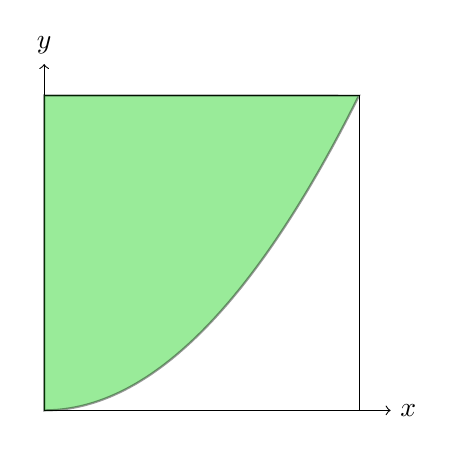
\begin{tikzpicture}[scale=4]
    \draw[->] (0,0) -- (1.1,0) node[right] {$x$};
    \draw[->] (0,0) -- (0,1.1) node[above] {$y$};
    \draw (1,0) -- (1,1) node {};
    \draw (0,1) -- (1,1) node {};
    \filldraw[thick,fill=green!80!black,opacity=.4] plot [smooth,domain=0:1] ({\x},{\x^2}) -- (0,1) -- cycle;
  \end{tikzpicture}
  \caption{$A$}
\end{figure}
\noindent
We kunnen nu de integraal spliten:
\[ \int_{0}^{1} \int_{x^{2}}^{1}f(x,y)\ dy\ dx \]
... en uitrekenen.
\begin{align*}
  \int_{0}^{1} \int_{x^{2}}^{1}3x^{2} + xy + 2y^{2}\ dy\ dx
  &= \int_{0}^{1} \left( 3x^{2}(1-x^{2}) + \frac{x}{2}(1-x^{4}) + (1-x^{6})\right)\ dx\\
  &= \int_{0}^{1}-x^{6}-\frac{1}{2}x^{5}-3x^{4}+3x^{2}+\frac{1}{2}x 1\ dx\\
  &= -\frac{1}{7} - \frac{1}{12} - \frac{3}{5} + 1 + \frac{1}{4} + 1\\
  &=  \frac{299}{210}
\end{align*}


\newpage
\section{Opzoeken in de tabel van de standaard normale verdeling}
Het is niet evident en niet uitgelegd hoe iets in de tabel van de standaard normale verdeling opgezocht kan worden. 
Hier daarom wat uitleg.

Allereerst is het belangrijk om te weten dat de getallen in de tabel zelf de kans $P(Z \le z)$ voorstel, waarbij $z$ wordt gegeven door de rand van de tabel.
De som van de waarde aan het begin van de rij en de waarde het begin van de kolom geeft u de $z$ waarvoor $P(Z \le z)$ in de tabel staat.

In de tabel staat natuurlijk niet de kans $P(Z \le z)$ voor alle mogelijke $z$.
Er staan alleen kansen in voor bepaalde $z \in \interval{0}{3.3}$ en enkel voor maximum twee cijfers na de komma.
De maker van de tabel ging er bovendien van uit dat u twee dingen weet:

\[ P(Z \le z) = 1 - P(Z > z) \quad\text{ en }\quad P(Z \le z) = P(Z \ge -z) \]

Merk op dat die eerste gelijkheid strikt klopt, maar omdat we de resultaten toch al niet exact zijn (door afrondingen) maken we er eveneens het volgende van:
\footnote{Ja. Ik weet het. Ik vind het ook lelijk maar dat is nu eenmaal waar statistici zich mee bezig houden.}
\[ P(Z \le z) = 1 - P(Z \le z) \]
Aan de hand van deze twee regels kunnen we uit de tabel nog veel meer informatie halen.

We kunnen bovendien, mits een beetje gefoefel, de tabel ook gebruiken om, gegeven een bepaalde kans $P(Z \le z)$ de $z$ te bepalen. 

\subsection*{Abstract}
\subsubsection*{Vraag}
\begin{itemize}
\item 
  \begin{enumerate}
  \item Bepaal $P(Z \le z)$ voor $z \in\interval{0}{3.3}$
  \item Bepaal $P(Z \ge z)$ voor $z \in\interval{0}{3.3}$
  \item Bepaal $P(Z \le z)$ voor $z \in\interval{-3.3}{0}$
  \item Bepaal $P(Z \ge z)$ voor $z \in\interval{-3.3}{0}$
  \end{enumerate}
\item
  \begin{itemize}
  \item Bepaal $z$ zodat $P(Z \le z) = p$ geldt met $p \in \interval{0.5}{1}$ 
  \item Bepaal $z$ zodat $P(Z \ge z) = p$ geldt met $p \in \interval{0.5}{1}$
  \item Bepaal $z$ zodat $P(Z \le z) = p$ geldt met $p \in \interval{0}{0.5}$
  \item Bepaal $z$ zodat $P(Z \ge z) = p$ geldt met $p \in \interval{0}{0.5}$
  \end{itemize}
\end{itemize}

\subsubsection*{Antwoord}
\begin{itemize}
\item 
  \begin{enumerate}
  \item Lees $P(Z \le z)$ af.
  \item Lees $P(Z \le z)$ af. Het resultaat is $1-P(Z \le z)$.
  \item Lees $P(Z \le -z)$ af. Het resultaat is $1-P(Z \le -z)$.
  \item Lees $P(Z \le -z)$ af. Dit is meteen het resultaat.
  \end{enumerate}
\item
  \begin{enumerate}
  \item Zoek $p$ in de tabel en tel de hoofdingen op.
  \item Zoek $p$ in de tabel en tel de hoofdingen op om $-z$ te bekomen.
  \item Zoek $1-p$ in de tabel en tel de hoofdingen op om $-z$ te bekomen.
  \item Zoek $1-p$ in de tabel en tel de hoofdingen op om $z$ te bekomen.
  \end{enumerate}
\end{itemize}


\subsection*{Voorbeeld}
\subsubsection*{Vraag}
\begin{itemize}
\item
  \begin{enumerate}
  \item Bepaal $P(Z \le 1.25)$
  \item Bepaal $P(Z \ge 1.25)$
  \item Bepaal $P(Z \le -0.3)$
  \item Bepaal $P(Z \ge -0.3)$
  \end{enumerate}
\item
  \begin{enumerate}
  \item Bepaal $z$ zodat $P(Z \le z) = 0.6$ geldt
  \item Bepaal $z$ zodat $P(Z \ge z) = 0.6$ geldt
  \item Bepaal $z$ zodat $P(Z \le z) = 0.2$ geldt
  \item Bepaal $z$ zodat $P(Z \ge z) = 0.2$ geldt.
  \end{enumerate}
\end{itemize}
\subsubsection*{Antwoord}
\begin{itemize}
\item
  \begin{enumerate}
  \item $P(Z \le 1.25) = 0.894$
  \item $P(Z \ge 1.25) = 1-P(Z \le 1.25) = 1- 0.894 = 0.106$
  \item $P(Z \le -0.3) = P(Z \ge 0.3) = 1- P(Z \le 0.3) = 1-0.619 = 0.381$
  \item $P(Z \ge -0.3) = P(Z \le 0.3) = 0.619$
  \end{enumerate}
\item
  \begin{enumerate}
  \item $P(Z \le z) = 0.6 \Rightarrow z = 0.25$
  \item $P(Z \ge z) = 0.6 \Rightarrow P(Z \le -z) = 0.6 \Rightarrow -z = 0.25 \Rightarrow z = -0.25$ 
  \item $P(Z \le z) = 0.2 \Rightarrow 1-P(Z \ge z) = 0.2 \Rightarrow P(Z \ge z) = 0.8 \Rightarrow P(Z \le -z) = 0.8 \Rightarrow -z = 0.84 \Rightarrow z = -0.84$
  \item $P(Z \ge z) = 0.2 \Rightarrow 1-P(Z \le z) = 0.2 \Rightarrow P(Z \le z) = 0.8 \Rightarrow z = 0.8$
  \end{enumerate}
\end{itemize}

\newpage
\section{Verwachtingswaarde en variantie berekenen aan de hand van een MGF}
\subsection*{Abstract}
\subsubsection*{Vraag}
Gegeven de momentgenererende functie $M_{X}(t)$ van een stochastische variabele $X$, bepaal de verwachtingswaarde en de variantie van $X$.

\subsubsection*{Antwoord}
De verwachtingswaarde is gelijk aan het eerste ruwe moment.
\[ E[X] = \alpha_{1} \]
De variantie is gelijk aan het eerste centrale moment, dat we overigens kunnen schrijven in functie van het eerste ruwe en het tweede ruwe moment:
\[ Var[X] = \mu_{1}(X) = \alpha_{2}(X) - \alpha_{1}(X)^{2} = E[X^{2}] - E[X]^{2} \]
De ruwe momenten kunnen we tenslotte vinden door de momentgenererende functie af te lijden en daarna te evalueren in nul.
\[ \alpha_{k} = \left.\frac{d^{k}}{dt^{k}}M_{X}(t)\right|_{t=0} \]

\subsection*{Voorbeeld}
\subsubsection*{Vraag}
Zij $X$ een stochastische variabele met de volgende momentgenererende functie:
\[ M_{X}(t) = e^{-5t} \]
Bepaal de verwachtingswaarde en de variantie van $X$.

\subsubsection*{Antwoord}
We berekenen eerst de afgeleide van $M_{X}(t)$:
\[ \frac{d}{dt}M_{X}(t) = -5e^{-5t} \]
In $t=0$ is dit $-5$.
De verwachtinsgwaarde van $X$ is dus $-5$.\\
Nu de tweede afgeleide van $M_{X}(t)$:
\[ \frac{d^{2}}{dt^{2}}M_{X}(t) = \frac{d}{dt} -5e^{-5t} = 25e^{-5t} \]
In $t=0$ is dit $25$.
De variantie van $X$ kunnen we nu eenvoudig berekenen:
\[ Var[X] = 25 - (-5)^{2} = 0 \]

\end{document}

%%% Local Variables:
%%% mode: latex
%%% TeX-master: t
%%% End:
